\begin{question}
\noindent Triangle $T$ has vertices $A(-5,1)$, $B(-5,3)$ and $C(-2,1)$.

\begin{center}
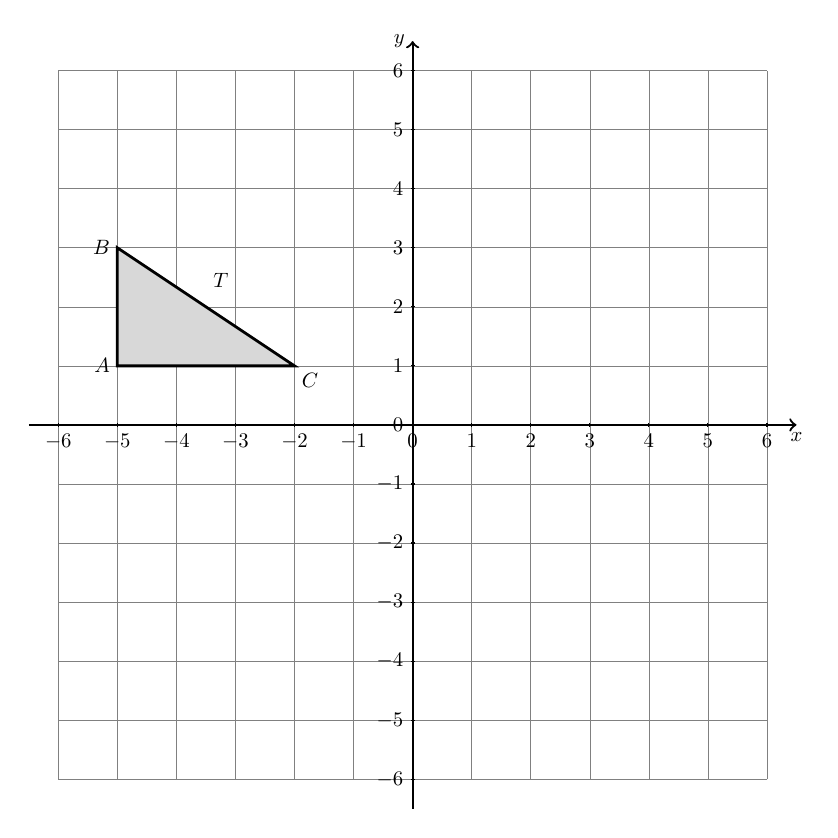
\begin{tikzpicture}[scale=0.75, transform shape]
    % Define axis scale
    \def\axisLimit{6}

    \definecolor{borderColour}{HTML}{000000}
    \definecolor{fillColourT}{HTML}{D8D8D8}
    \definecolor{fillColourU}{HTML}{BFD8FF}

    % Draw grid
    \draw[step=1cm,gray,very thin] (-\axisLimit,-\axisLimit) grid (\axisLimit,\axisLimit);

    % Draw axes
    \draw[thick,->] (-\axisLimit-0.5,0) -- (\axisLimit+0.5,0) node[anchor=north] {$x$};
    \draw[thick,->] (0,-\axisLimit-0.5) -- (0,\axisLimit+0.5) node[anchor=east] {$y$};

    % Label x-axis and y-axis
    \foreach \x in {-\axisLimit,...,\axisLimit}
        \draw (\x cm,1pt) -- (\x cm,-1pt) node[anchor=north] {$\x$};
    \foreach \y in {-\axisLimit,...,\axisLimit}
        \draw (1pt,\y cm) -- (-1pt,\y cm) node[anchor=east] {$\y$};

    % Draw triangle T
    \draw[fill=fillColourT, draw=borderColour, line width=1pt] (-5,1) -- (-5,3) -- (-2,1) -- cycle;
    \node[left] at (-5,1) {$A$};
    \node[left] at (-5,3) {$B$};
    \node[below right] at (-2,1) {$C$};
    \node[above right] at (-3.5,2.2) {$T$};

\end{tikzpicture}
\end{center}

\begin{enumerate}
    \item[(a)] Triangle $T$ is translated by the vector $\begin{pmatrix} 7 \\ -4 \end{pmatrix}$ to give triangle $U$.

    Find the coordinates of the vertices of triangle $U$.

    \vspace{3cm}
    \answerplain{1}

    \item[(b)] Triangle $U$ is then reflected in the line $x = 0$ to give triangle $V$.

    Describe fully the \textbf{single} transformation that maps triangle $T$ directly onto triangle $V$.

    \vspace{4.5cm}
    \answerlines{3}{2}
\end{enumerate}
\end{question}